\subsection{Testing the Questionnaire Language}

\subsubsection{Creating a Launch Configuration}

In order to test the language and the editor we need to deploy the developed
plugins within another Eclipse instance. For testing the easiest way is start a
so-called Runtime Instance.

Open the dialog \emph{Run / Run Configurations} and select the node \emph{Eclipse
Application} from the left tree widget and press the icon with the +
sign to create a new Launch Config.

You could leave the defaults here or change the name and location like in the
screenshot.

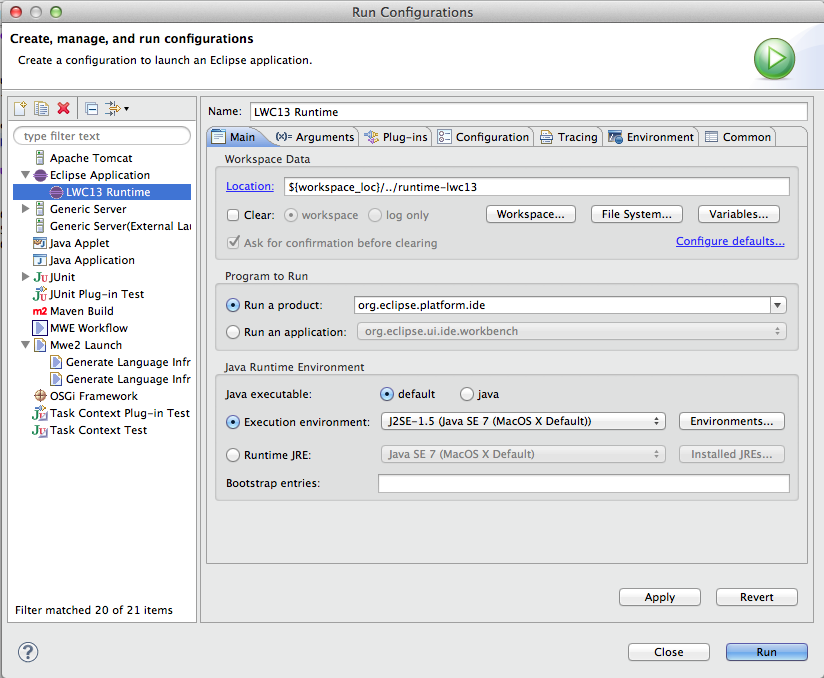
\includegraphics[width=17cm]{./images/chapter01/LaunchConfig.png}

Now switch to the Arguments page and enter in the ``VM arguments'' text box:
\begin{lstlisting}
-Xms40m -Xmx512m -XX:MaxPermSize=150m
\end{lstlisting}
Especially important is the MaxPermSize setting, since the default size of the
PermGen space of the VM (64MB) often is not enough.

Now press the \emph{``Run''} button. Another Eclipse instance will start with an
empty workspace. Close the Welcome window.


\subsubsection{Create Test Project}

In the Runtime Workspace create a new Java Project with name ``QLTest''.

Select the \texttt{/src} folder and create a new file
\texttt{``housepurchase.ql''}. Once you have created the file a popup dialog
will appear to ask, if you would like to add the Xtext nature on this project.
Answer with ``Yes''.

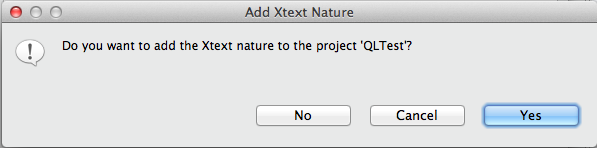
\includegraphics[width=12cm]{./images/chapter01/AddXtextNature.png}

From now on your project will be considered to contain files that Xtext should
recognize (\texttt{.ql} files). Projects having the Xtext nature will be processed by the
Xtext Builder when building projects, other projects are ignored. The Xtext
Builder indexes the Xtext based resources, links the cross-references in the
editor, and validates the model files. On errors, resource markers are created
which can be seen in the editor and the \emph{Problems View}.

